% !TeX TS-program = xelatex
% !BIB TS-program = bibtex

% Full instructions available at:
% https://github.com/pcafrica/focus-beamertheme

\documentclass{beamer}
\usetheme[nofirafonts]{focus}
\usefonttheme{serif}

\usepackage{tkz-graph}
\usepackage{booktabs}
\usepackage{fontawesome5}
\usepackage[cache=false]{minted}

% Tikz graph config
\tikzstyle{vertex}=[auto=left,circle,fill=black!25,minimum size=20pt,inner sep=0pt]

\title{Solving Bomberman}
\subtitle{\large with Q-table and Neural Networks}
\author{\small Behrooz Montazeran\texorpdfstring{\\}{,} Jannis Heising\texorpdfstring{\\}{,} Tomáš Sláma}
\titlegraphic{
\includegraphics[scale=20]{demolitionist.png}}
\date{28. 11. 2023}

\newcommand{\faEyeRegular}{\faEye[regular]}

\setbeamertemplate{caption}[numbered]

% Footline info is printed only if [numbering=fullbar].
%\footlineinfo{Custom footline text}

\begin{document}
\begin{frame}
	\maketitle
\end{frame}

\section{Introduction}

\begin{frame}{Problem Statement}
	\pause

	\begin{itemize}
		\item \textbf{6 actions} -- 5 movement directions + place bomb
		\item destructible crates, indestructible walls
		\item \textbf{+1} for coin, \textbf{+5} for killing opponent
	\end{itemize}
	\vfill
	\begin{center}
		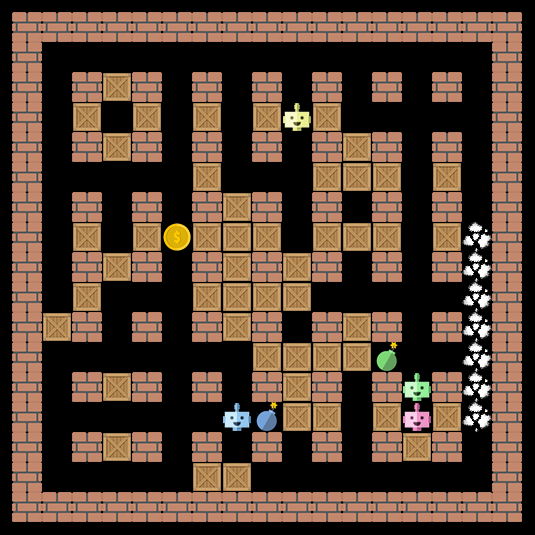
\includegraphics[width=0.4\linewidth]{bomberman_example.png}
	\end{center}
\end{frame}

\begin{frame}{Available Methods}
	\pause

	\textbf{Q-learning} -- optimizing action-value Q-function:
	\begin{itemize}
		\item \textbf{Q-table:} store each input/output in a table
		\item \textbf{Neural Network:} learn function via a neural network
	\end{itemize}

	\vspace{1.2em}
	\pause

	Updating Q-values:
	\begin{itemize}
		\item \textbf{SARSA:} TODO
		\item \textbf{TD:} TODO
		\item \textbf{n-step TD:} TODO
	\end{itemize}

	\vspace{1.2em}
	\pause

	Stability can be improved with policy/target model:
	\begin{itemize}
		\item \textbf{target}: trained on the results of actions
		\item \textbf{policy}: updated slowly / replaced periodically
	\end{itemize}
\end{frame}

\begin{frame}{Infrastructure}
	\pause

	Evaluation with \mintinline{text}{elo.py}:
	\begin{itemize}
		\item comparing relative strengths of agents using the elo system
		\item agents start with $1\;000$ elo, updated after win/loss/draw
	\end{itemize}

	\vspace{1.2em}
	\pause

	Training with \mintinline{text}{train.py}:
	\begin{itemize}
		\item subcommands for training traits (coin picking, agent hunting)
		\item periodically calculates strength with \mintinline{text}{elo.py}
		\item useful training flags: \mintinline{text}{--infinite <n>}, \mintinline{text}{--continue}
	\end{itemize}
\end{frame}

\begin{frame}[fragile]
	\frametitle{Training Command Example}
	\pause

\fontsize{7}{9}
\begin{minted}{python}
TASKS = {
    ...
    "complete": [
        # first learn to pick up coins
        (["--scenario", "coin-heaven", "--n-rounds", "100"], False),
        # then learn to hunt/evade the rule-based agent
        (["rule_based_agent", "--scenario", "empty", "--n-rounds", "1000"], False),
        # then learn to work with crates
        (["--scenario", "classic", "--n-rounds", "1000"], False),
        # then learn to work with crates + hard agent
        (["rule_based_agent", "--scenario", "classic", "--n-rounds", "200"], True),
        # then learn to work with crates + really hard agent
        (["binary_agent_v3", "--scenario", "classic", "--n-rounds", "200"], True),
        # finally play against itself (None gets substituted)
        ([None, "--scenario", "classic", "--n-rounds", "200"], True),
    ],
    ...
}
\end{minted}
\end{frame}

\section{Neural Networks}

\begin{frame}{Overview}
	\pause

	\textbf{Network structure:} fully connected layers with ReLU
	\begin{itemize}
		\item uses TD for Q-value updating
	\end{itemize}

	\vspace{1.2em}
	\pause

	Main idea -- carefully crafted binary state vector:
	\begin{itemize}
		\item[]\hspace{-1.8em} $\phantom{0}1 \ldots \phantom{0}5$: direction to the nearest \textbf{coin}
		\item[]\hspace{-1.8em} $\phantom{0}6 \ldots 10$: direction to the nearest \textbf{crate}
		\item[]\hspace{-1.8em} $11 \ldots 15$: direction to where a bomb will \textbf{kill opponent}
		\item[]\hspace{-1.8em} $16 \ldots 20$: direction to \textbf{safety} (if in danger of dying)
		\item[]\hspace{-1.8em} $\phantom{06 \ldots {}}21$: \textbf{can place a bomb} and there is a way to escape it
	\end{itemize}

	\vspace{1.2em}
	\pause

	Calculated by \textbf{searching state space} (other players stand still)
	\begin{itemize}
		\item[$\Rightarrow$] finds path even in ongoing explosions
		\item[$\Rightarrow$] shortest on-board path \(\neq\) shortest path stepwise
	\end{itemize}
\end{frame}

\begin{frame}{Q-vector example (1)}
	\pause
	\begin{figure}[t]
			\centering
			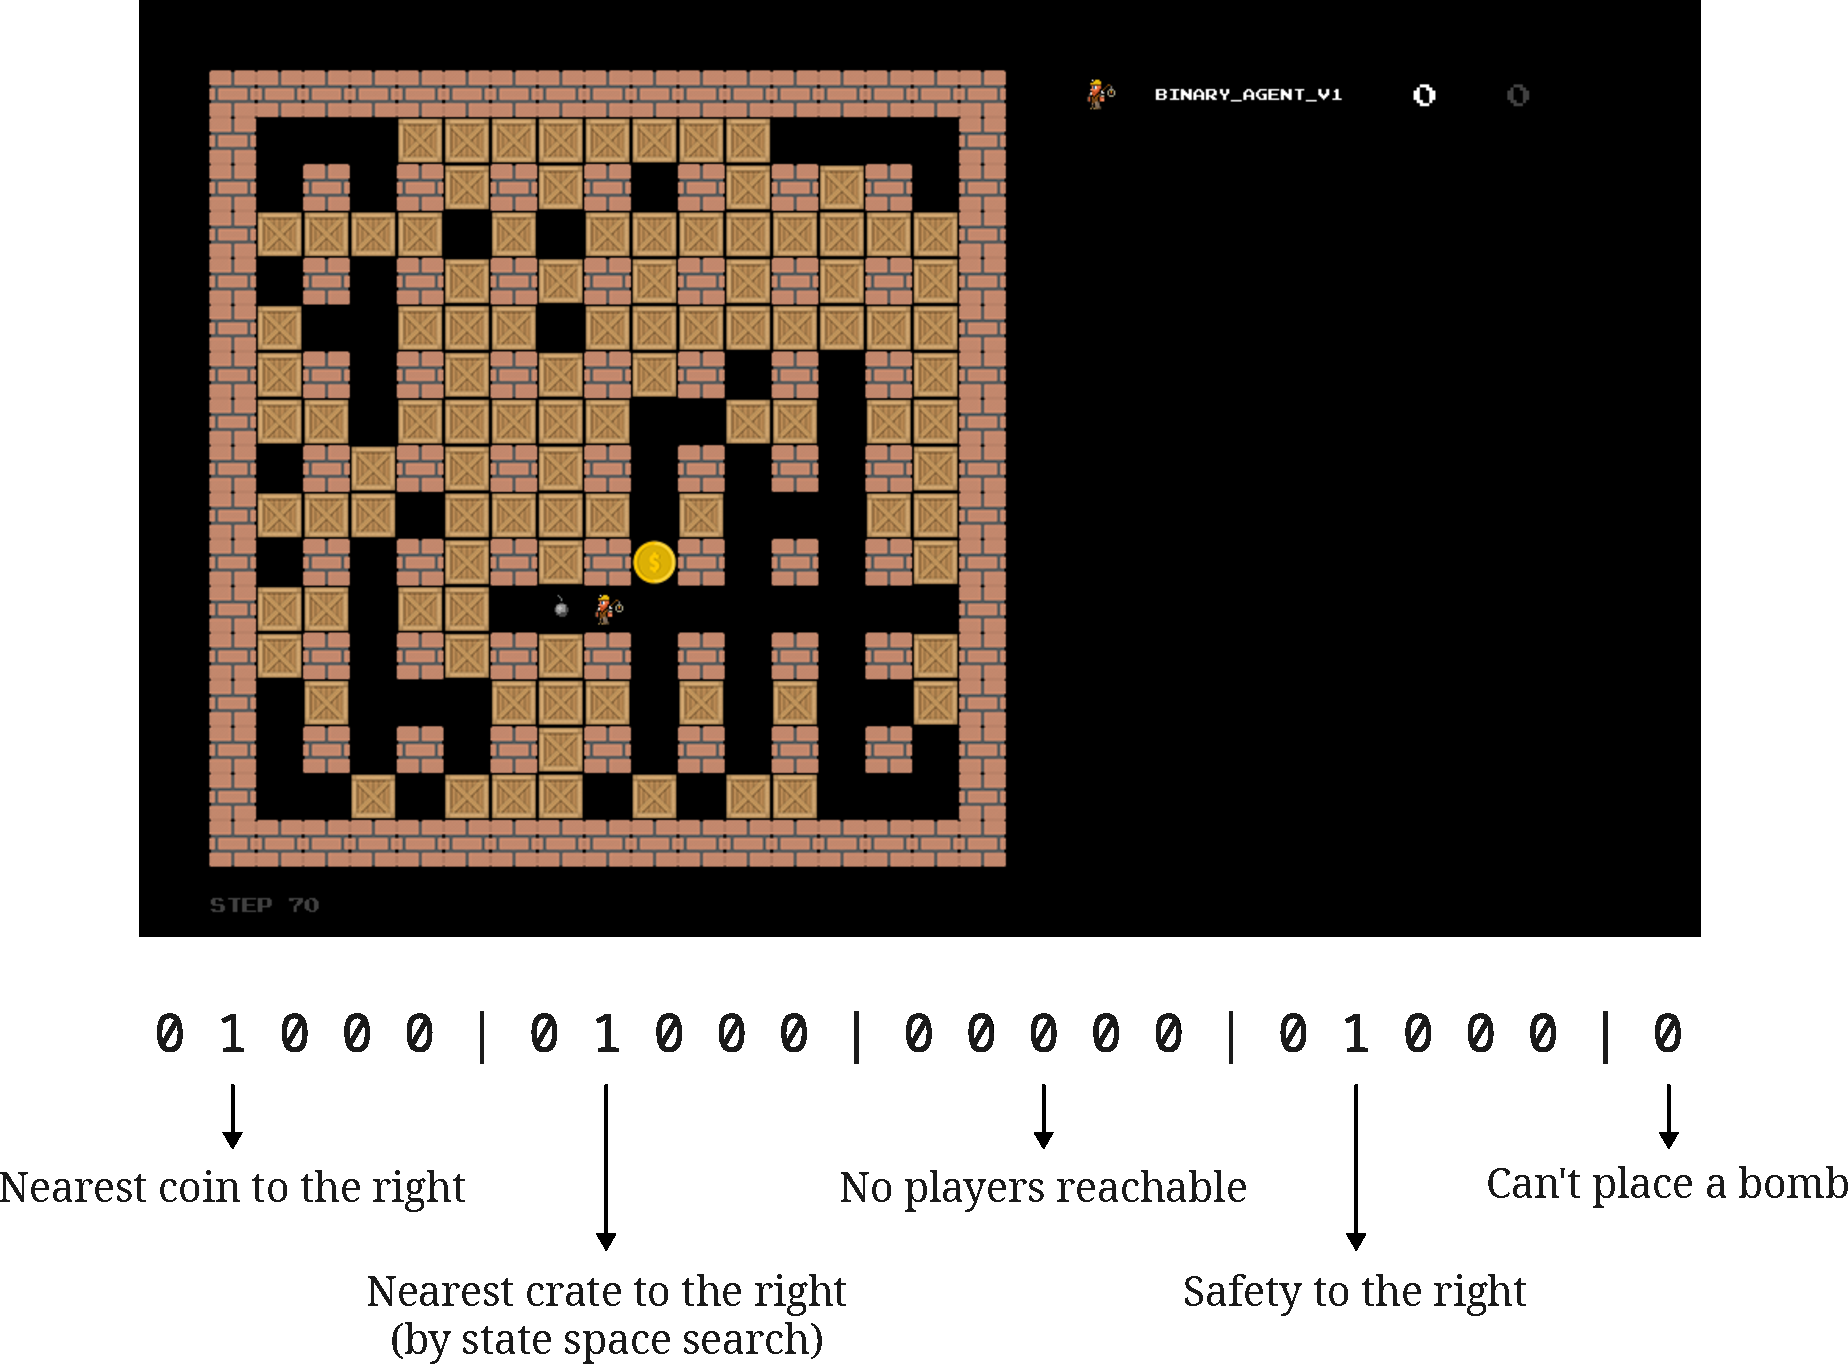
\includegraphics[width=.8\linewidth]{q-vector.pdf}
	\end{figure}
\end{frame}

\begin{frame}{Q-vector example (2)}
	\pause
	\begin{figure}[t]
			\centering
			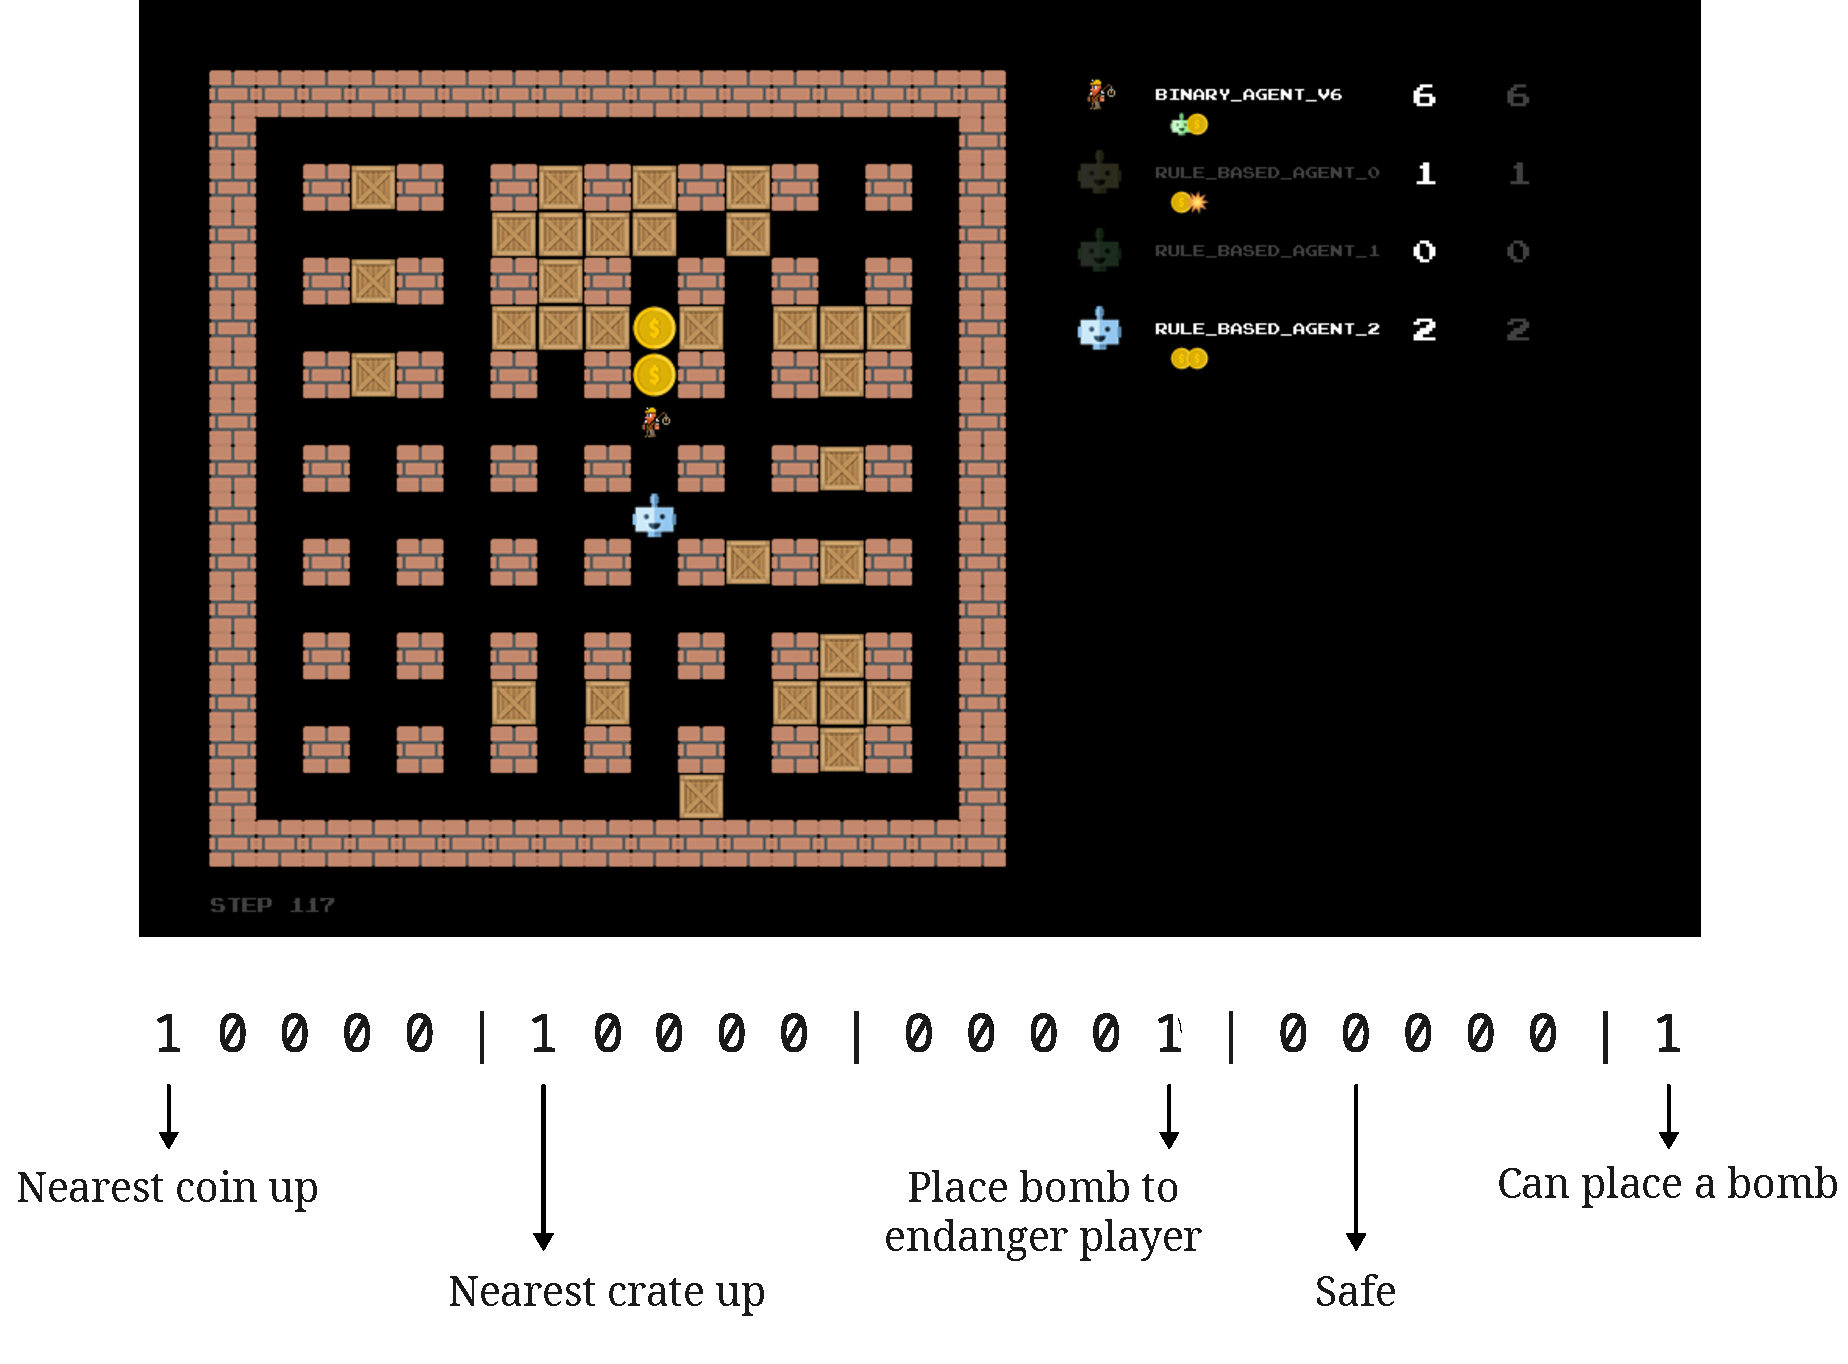
\includegraphics[width=.8\linewidth]{q-vector-2.pdf}
	\end{figure}
\end{frame}

\begin{frame}[fragile]
	\frametitle{Training Parameters}
	\pause
	\vspace{-1.3em}% not nice
	\begin{minipage}[t]{.5\textwidth}
\small
\underline{\textbf{Hyperparameters}}
\fontsize{6}{8}
\begin{minted}{python}
BATCH_SIZE = 256
MEMORY_SIZE = 1000

# chances of picking random action
EPS_START = 0.99
EPS_END = 0.05
EPS_DECAY = 10

# (soft) update rate of target network
TAU = 1e-3

# LR of the optimizer
LR = 1e-4

# discount for future states
GAMMA = 0.99

OPTIMIZER = optim.Adam
LAYER_SIZES = [1024, 1024]
\end{minted}
\end{minipage}%
	\begin{minipage}[t]{.5\textwidth}
\small
\underline{\textbf{Event Rewards}}
\fontsize{6}{8}
\begin{minted}{python}
# hunt coins
MOVED_TOWARD_COIN: 50
DID_NOT_MOVE_TOWARD_COIN: -100

# hunt people
MOVED_TOWARD_PLAYER: 25
DID_NOT_MOVE_TOWARD_PLAYER: -10

# blow up crates
MOVED_TOWARD_CRATE: 1

# basic stuff
e.INVALID_ACTION: -100
DID_NOT_MOVE_TOWARD_SAFETY: -500

# be active!
USELESS_WAIT: -100

# meaningful bombs
PLACED_USEFUL_BOMB: 50
PLACED_SUPER_USEFUL_BOMB: 150
DID_NOT_PLACE_USEFUL_BOMB: -500
\end{minted}
\end{minipage}%
\end{frame}

\begin{frame}[fragile]
	\frametitle{Training Loop}
	\pause

	\begin{enumerate}
			\item \texttt{train.py} with the \texttt{"complete"} task and \texttt{--infinite 2}
			\item pick the best-performing model based on calculated elo
			\item decrease \texttt{EPS\_START}, \texttt{EPS\_END}, \texttt{TAU} and \texttt{LR} hyperparameters
			\item go to step 1 (with \texttt{--continue} to not overwrite the model)
	\end{enumerate}

	\pause
	\begin{figure}[t]
			\centering
			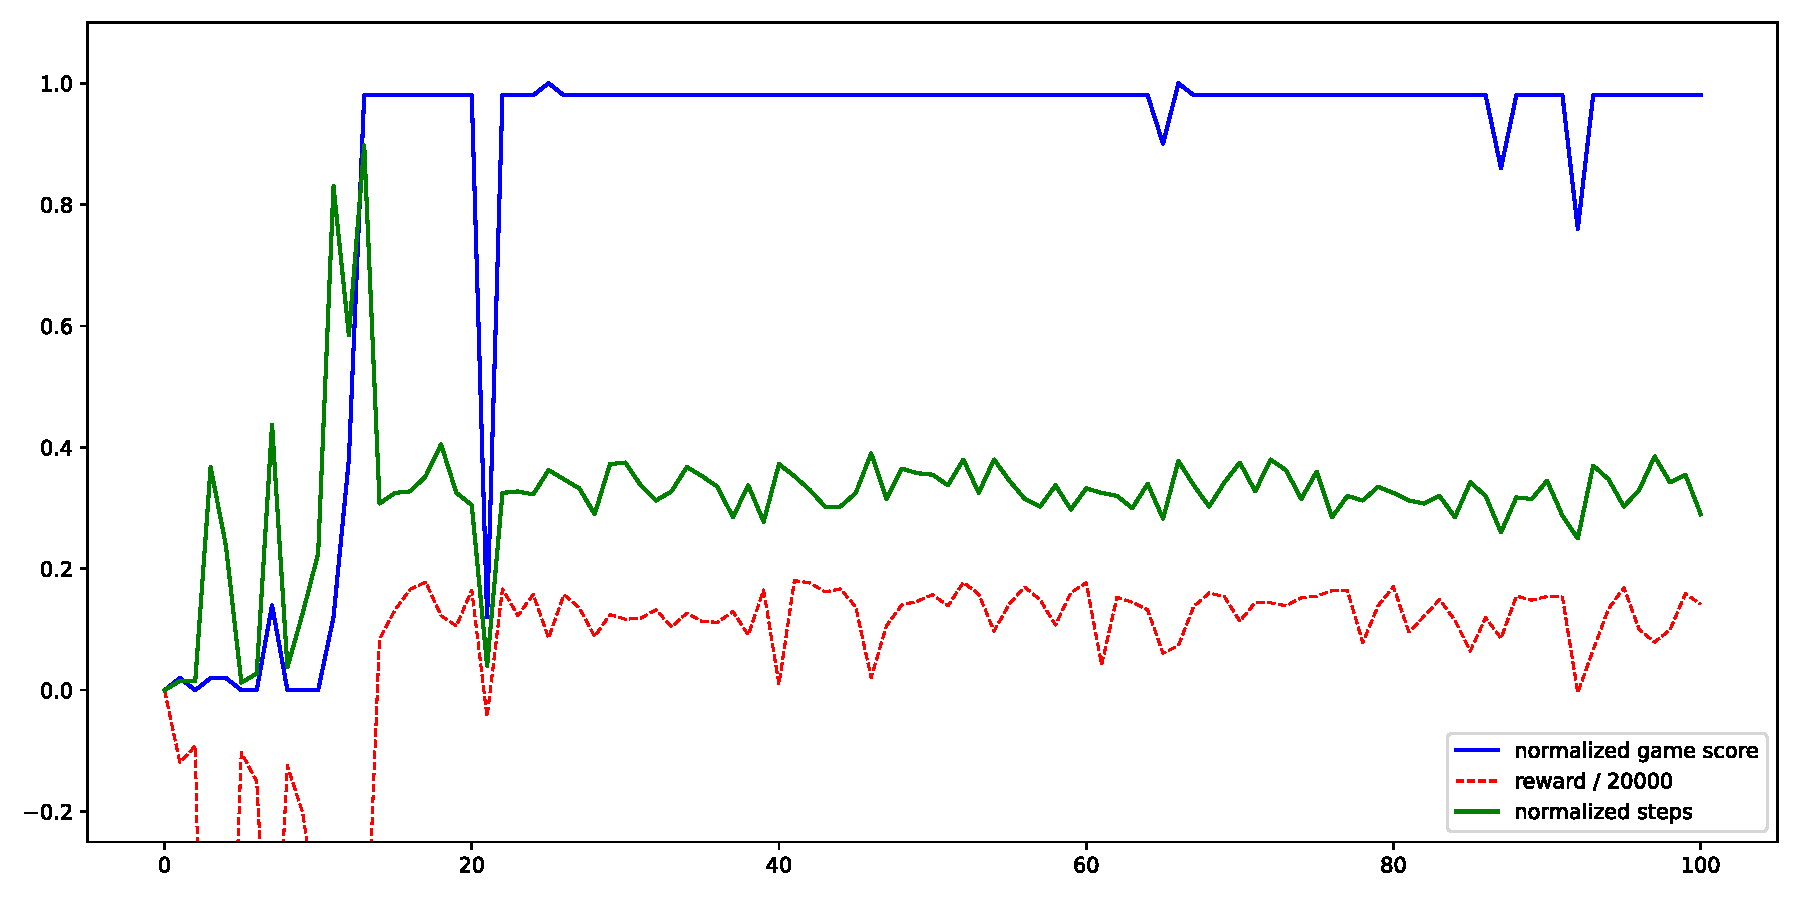
\includegraphics[width=.8\linewidth]{coins.pdf}
	\end{figure}
\end{frame}

\section{Q-table}

\begin{frame}{Overview}
	TODO

	\pause

	More TODO
\end{frame}

\section{Conclusion}

\begin{frame}[fragile]
	\frametitle{Results}
	\pause

	\begin{figure}[t]
			\centering
			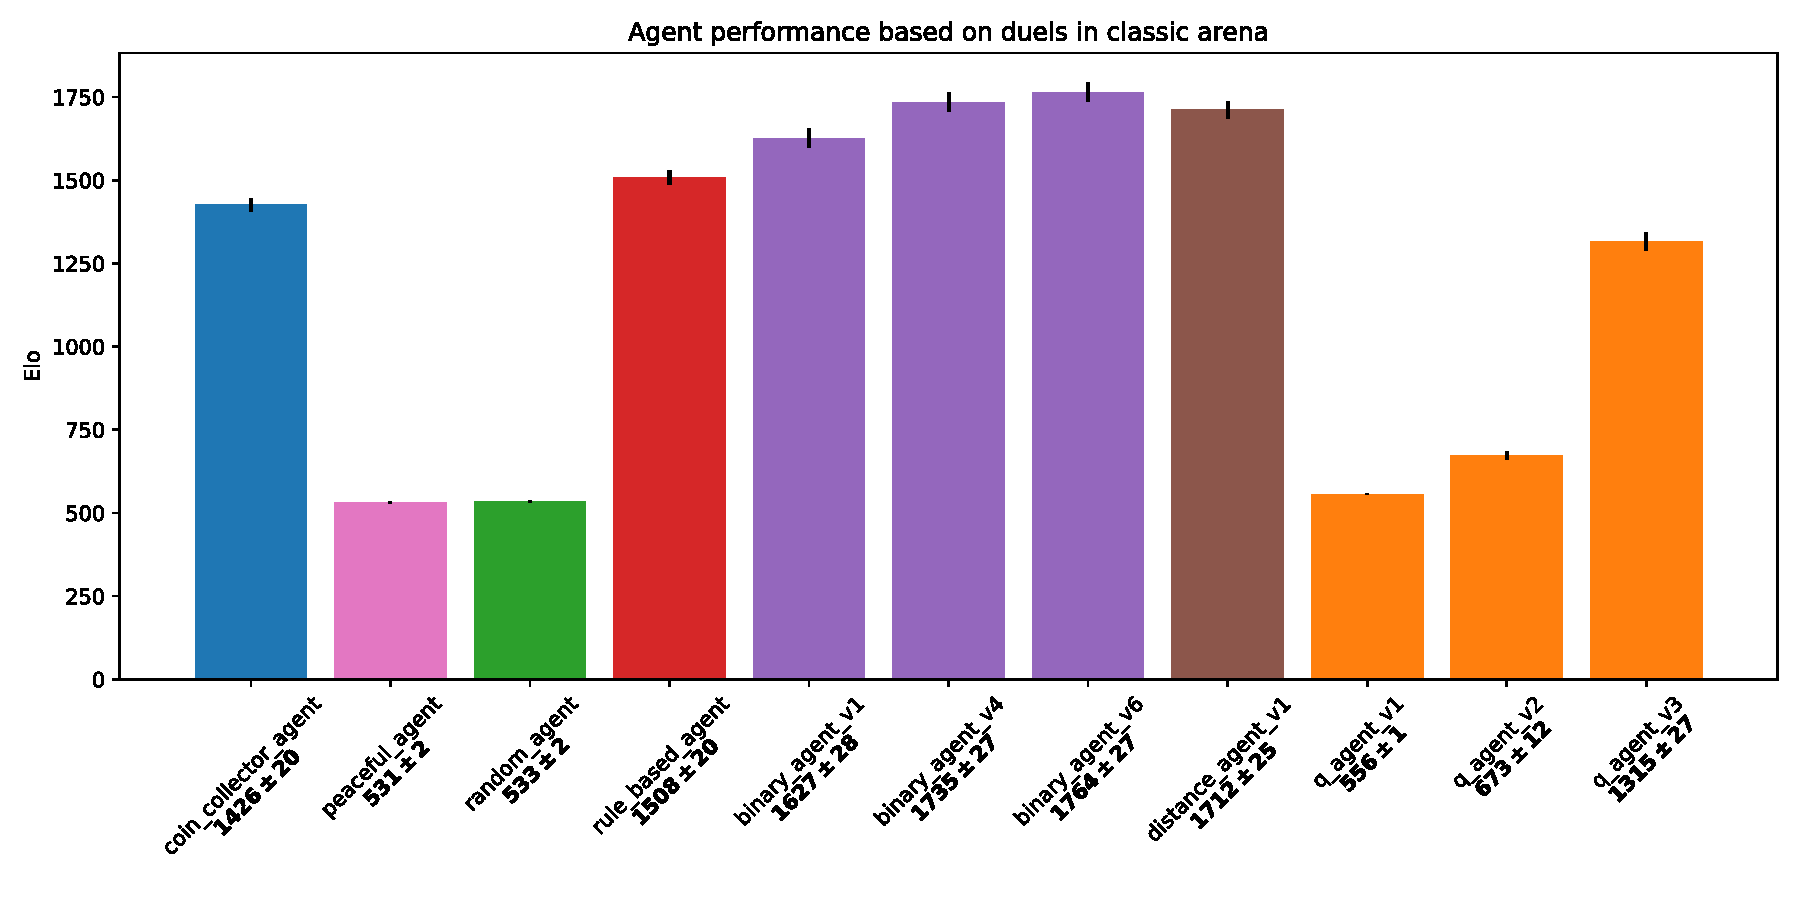
\includegraphics[width=1\linewidth]{elo.pdf}
	\end{figure}
\end{frame}


\begin{frame}[focus]
	Thanks for your attention!\\[0.2em]
	\small Special thanks to Ullrich Köthe and tutors\\[1.5em]
	
\includegraphics[scale=0.27]{xkcd.pdf}
\end{frame}

\appendix
\begin{frame}{References}
	\nocite{*}
	\bibliography{bibliography}
	\bibliographystyle{apalike}
\end{frame}
\end{document}
